\documentclass[11pt, twoside]{article} %iniciación del documento de tipo artículo, con tamaño de letra 11pt.
\usepackage[a4paper,total={6in, 8in},left=25mm, asymmetric]{geometry} %Cambio en los bordes y margenes del documento

\usepackage{fancyhdr} %Paquete para organizar y añadir header con los nombres

\usepackage{amsmath}

\usepackage[spanish,es-tabla,es-nodecimaldot]{babel}
\usepackage{tabularx}
\usepackage{booktabs}

\usepackage{caption}

\usepackage{graphicx}
\usepackage[hidelinks]{hyperref}
\usepackage{macro}

\fancypagestyle{main}{
    \fancyhf{}
    \fancyhead[L]{\thepage}
    \fancyhead[RO]{ZhuoZhuo L.}
    \renewcommand{\headrulewidth}{.4pt}
    \setlength{\headheight}{52pt}
}

\pagestyle{empty}

\begin{document}

\begin{figure}[h!]
    \minipage{0.87\textwidth}
	
\includegraphics[width=3cm]{Icons/ugr.jpg}
	\endminipage
    \minipage{0.87\textwidth}
	
\includegraphics[height = 2.5cm, width=3cm]{Icons/facultad_ciencias.png}
	\endminipage
	%%\vspace{-1cm}
\end{figure}

\vspace{0.3cm}

\begin{center}
    \Huge \textbf{Física Computacional}\\
    		\vspace{0.4cm}
    \LARGE \textbf{Voluntario 1:}  
    Simulación con dinámica molecular de un gas con un potencial de Lennard-Jones
\end{center}

\vspace{1cm}

\vspace{1cm}

\begin{center}
    \large \textbf{Resumen}\\
    		\vspace{0.2cm}
    \normalsize
    En este informe tenemos como objetivo ...

\end{center}

\vspace{1cm}

\begin{flushright}
    \large Zhuo Zhuo Liu 
    \\
    \vspace{0.4cm}
    \textbf{Grado en Física}
\end{flushright}

\newpage

\setcounter{page}{0}
\tableofcontents
\newpage

\pagestyle{main}

\section{Introducción}

\section{Planteamiento del problema}

Para poder 

\subsection{Condiciones iniciales}
Al introducir las condiciones iniciales del sistema, debemos de tener cuidado de
no colocar 2 partículas muy cercas entre ellas inicialmente, ya que puede provocar
que las partículas adquieran mucha velocidad. 

Para ello consideramos una cuadrícula separada por una distancia $L/5$ en ambos 
ejes, y permitimos que las partículas se desplace una distancia aleatoria entre 0 y 1
de dicha posición. Y una velocidad con dirección aleatoria, pero con módulo unidad.

\subsection{Condiciones de contorno}

Para introducir la condición de contorno bidimensional periódica empleamos 
2 funciones, una para la posición de las partículas, y la otra para la 
distancia entre partículas. Pero ambos seguirán la misma lógica.

Comenzando para la posición de las partículas, se tiene que si una partícula en su
nueva posición tiene una coordenada mayor que $L$ o menor que 0, entonces se le 
restará o sumará $L$ a dicha coordenada dependiendo del caso. 

Mientras que para la distancia entre partículas, se tiene que si la distancia entre
partículas en una de las coordenadas es mayor que $L/2$, entonces se le restará 
$L$ a la distancia. Y aplicando lo mismo al caso contrario, cuando la distancia es
menor que $-L/2$.

Notar que se ha tenido que diferenciar en 2 funciones muy similares, pero con diferentes
condiciones, ya que el sistema no está centrado en 0. Si se hubiera centrado en 0, 
ambas funciones serían iguales.

Una vez tenida estas condiciones, ya podemos calcular la distancia entre partículas,
estas distancias será importantes tanto para calcular las fuerzas de interacción, como 
la energía potencial del sistema. 

Guardaremos estas distancias o mejor dicho los vectores que las unen en una matriz 
de dimensiones $N\times N\times 2$, donde $N$ es el número de partículas, y 2 indica
las dimensiones del espacio. El cálculo de estas distancias es sencillo, siendo la
resta entre las posiciones de las partículas. 

Podemos reducir el número de cálculos al notar que la matriz es antisimétrica, entonces el 
elemento $R_{ij}$ es igual a $-R_{ji}$, por lo que solo necesitamos calcular menos de 
la mitad de la matriz, y asignar el valor correspondiente a los otros elementos.

\subsection{Potencial Lennard-Jones}

Una vez tenido las funciones para imponer la condición de contorno y el cálculo de 
las distancias entre partículas, podemos calcular la fuerza de interacción entre 
partículas por el potencial de Lennard-Jones.

\begin{equation}
    V(r) = 4\epsilon\brackets{\parenthesis{\frac{\sigma}{R}}^{12}-
        \parenthesis{\frac{\sigma}{R}}^{12}}
    \label{eq:Lennard_Jones_potential}
\end{equation}

donde se ha usado $R$ en lugar de $r$, para coincidir en la notación empleada en 
el código.

\vspace{3mm}

Entonces la fuerza de interacción entre las partículas viene dado por:

\begin{equation}
    \vec{F}(\vec{R}) =  - 4\epsilon\brackets{6\parenthesis{\frac{\sigma}{R}}^{5}-
    12\parenthesis{\frac{\sigma}{R}}^{11}}
\end{equation}

Para calcular la aceleración de la partícula, se suma la fuerza de interacción con
todas las demás las partículas, y se divide por la masa.

Implementando en todo esto en la función que te devuelve la aceleración del sistema
en función de la posición de las partículas.


\subsection{Algoritmo de Verlet}

Por último solo queda añadir una función que nos permita calcular la nueva posición
de las partículas, y la nueva velocidad de las partículas. Para ello emplearemos el
algoritmo de Verlet. 

\section{Análisis de Resultados}

\subsection{Comparación con la distribución de Maxwell-Boltzmann}

Partiendo de las condiciones iniciales propuestas (20 átomos de Argón en una caja 
de $L=10$, y velocidades de módulo 1 con dirección aleatoria), se ha simulado el
experimento se ha simulado un tiempo $t = 50$, con un paso del tiempo 
$\Delta t = 0.002$.

La evolución del sistema puede visualizarse en formato gif, en el 

Representando la evolución de la energía cinética, potencial y total del sistema
a lo largo del tiempo, se obtiene la figura \ref{fig:energias}.

\begin{figure}[h!]
    \centering
    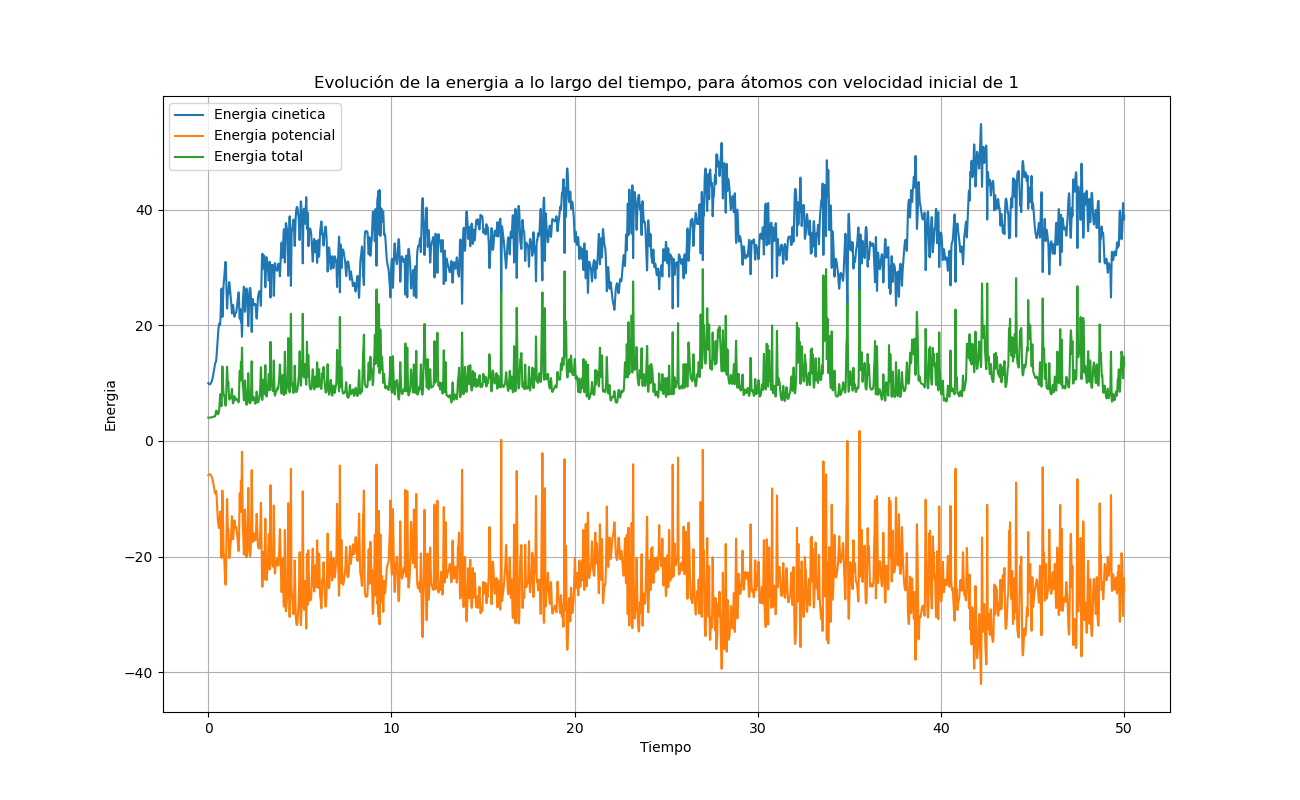
\includegraphics[width=\textwidth]{plots/energia_vel_init_1.png}
    \caption{Evolución de las energías del sistema}
    \label{fig:energias}
\end{figure}

La temperatura lo podemos calcular por el teorema de equipartición:

\begin{equation}
    k_B T = \frac{m}{2}\langle v_x^2 + v_y^2 \rangle
\end{equation}

donde considerando que $k_B =1$, y $m=1$, se tiene que la temperatura es igual a
$T = 1.$, 

Comparando la distribución de velocidades antes y despues de la relajación con la 
de Maxwell-Boltzmann,

\subsection{Ecuación de estado}

\subsection{Transición de fase sólido-líquido}
Para estudiar la transición de fase sólido-líquido, primero estudiaremos el estado
sólido, para ello se ha empleado un sistema de 16 partículas en una caja de 
$L=4$, con condiciones iniciales de una red cuadrada y en reposo. La idea es ver 
que el sistema evoluciona hasta un estado de equilibrio, donde se dispondrán 
en una estructura triangular.


De hecho este comportamiento se verificar para otras configuraciones iniciales, 
siempre que la temperatura del sistema sea lo suficientemente baja.

Entonces para ver la transición de fase, se irá aumentado la temperatura del sistema, 
es decir aumentado su velocidad en un factor $1.5$ en los tiempos 
$t=20, 30, 35$ y $45$.


El proceso anterior esta bien para observar el fenómeno de la transición de fase,
sin embargo, para estimar la temperatura crítica, se ha de calentar el sistema más lentamente
y dejando que el sistema se relaje.


\newpage

\appendix

\section{Tabla de valores}


\newpage

\section{Análisis de errores}


\end{document}
